\chapter{Results}\label{chap:results}

The following section describes the experimental setup, the used datasets and parameters and the experimental results achieved.

\section{Experimental Setup}



\begin{lstlisting}[language=bash, caption={Command used to count the number of .gv memory graph files generated by \textit{mem2graph} inside one of the servers mem2graph dataset directory.}]
    (py311) root@compute-container-rascoussie-d584d4794-lbm9r:~/onyr_phdtrack/mem2graph# find data/ -type f -name "*.gv" | wc -l
    104808
\end{lstlisting}

\section{Feature Engineering results}

\begin{figure}[H]\label{results:corr_matrices:kendall}
    \centering
    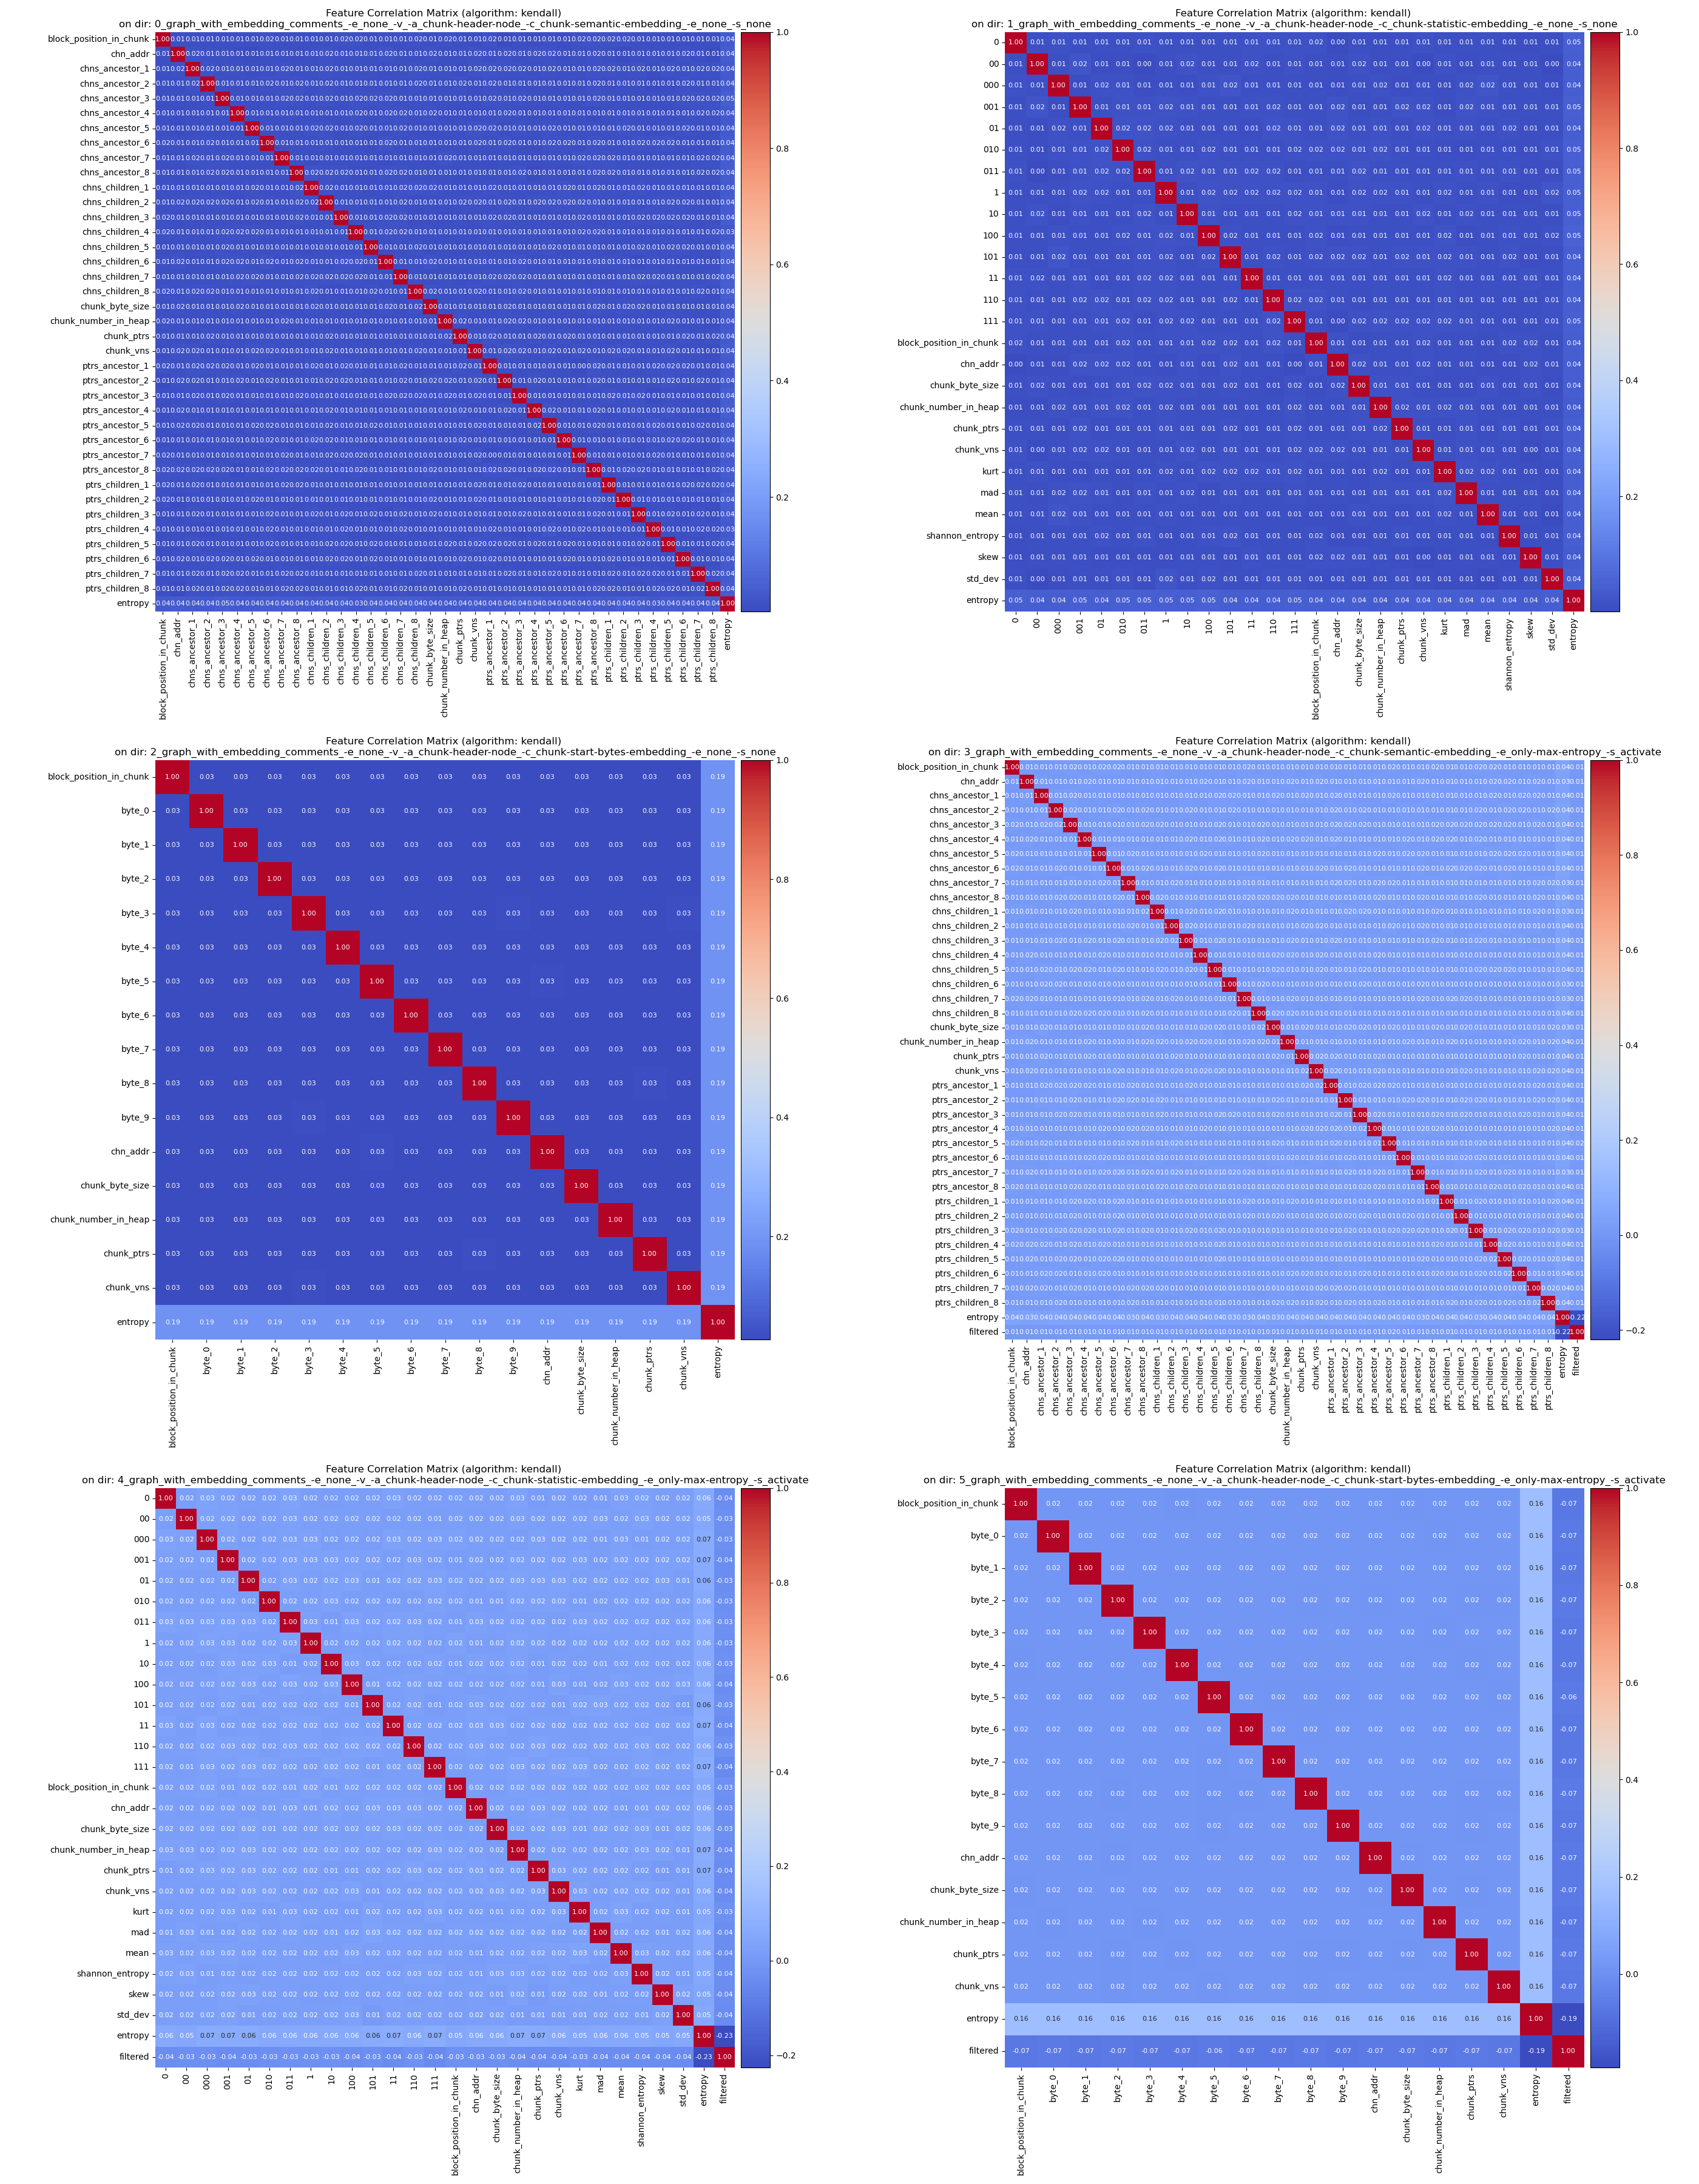
\includegraphics[width=16cm]{feature_engineering/concatenated_1_2023_10_24_kendall.png}
    \caption{Feature correlation matrices on the different Mem2Graph-generated datasets. Used algorithm: Kendall.}
\end{figure}

\begin{figure}[H]\label{results:corr_matrices:pearson}
    \centering
    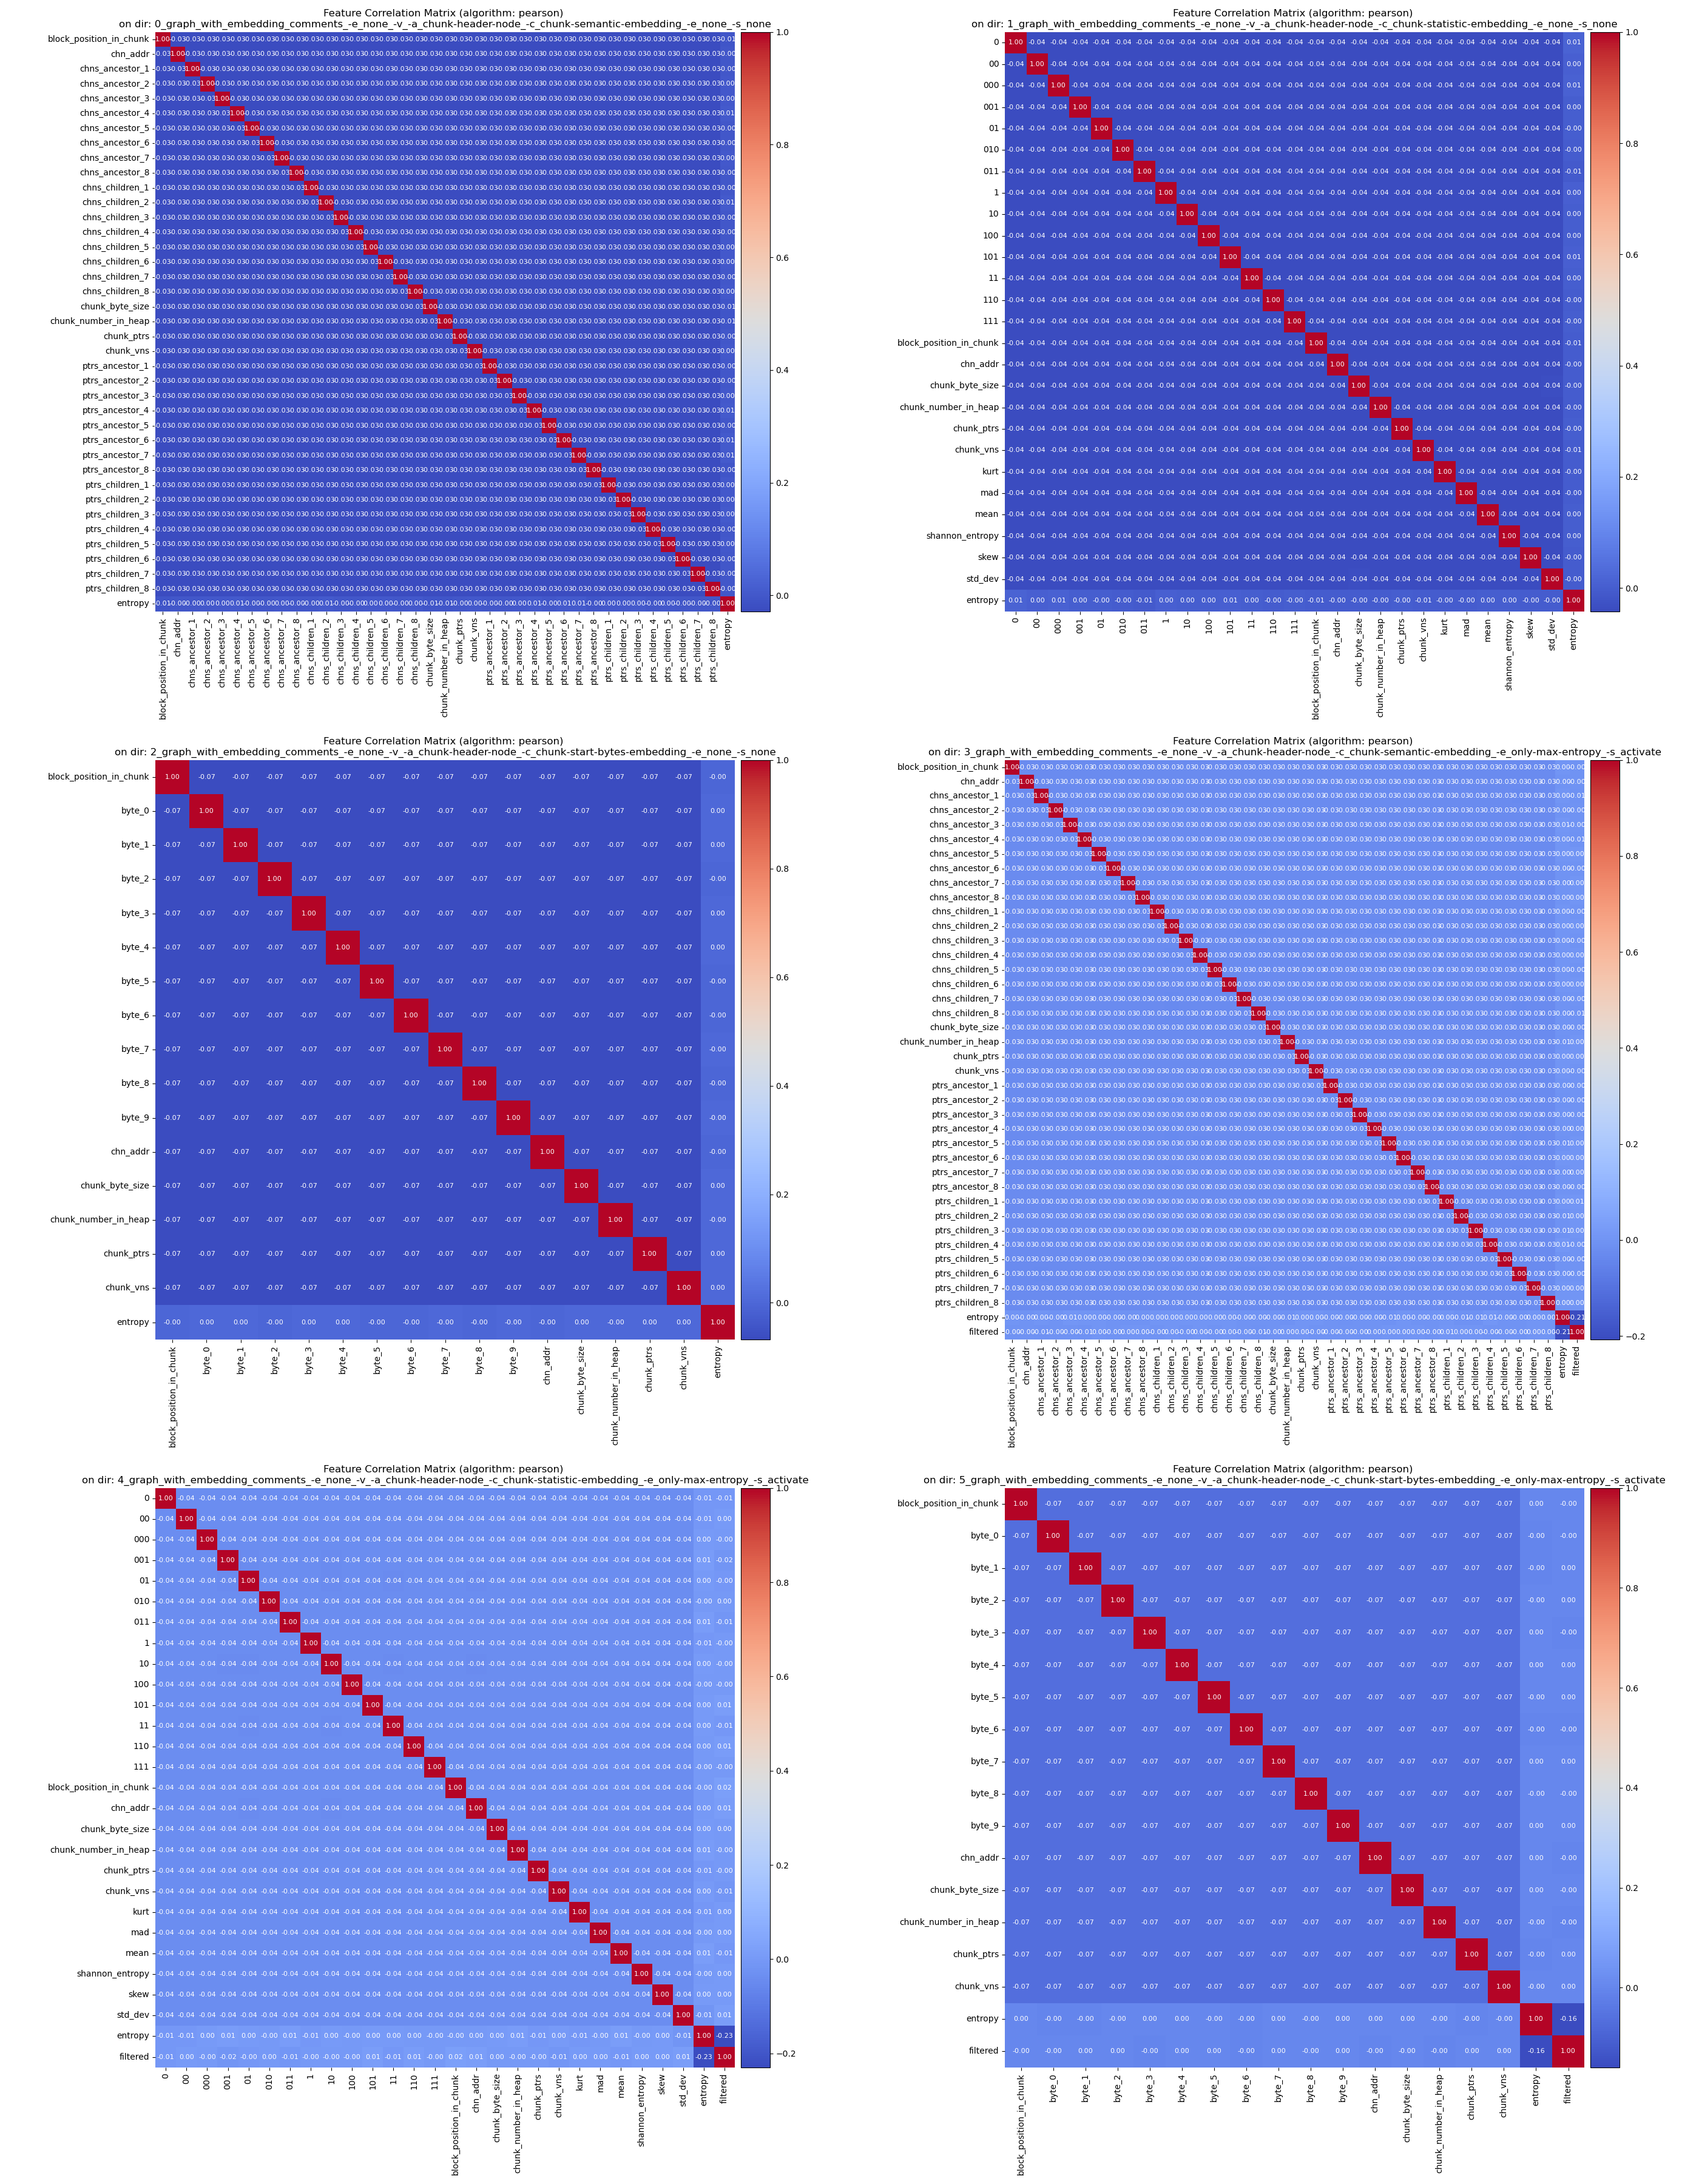
\includegraphics[width=16cm]{feature_engineering/concatenated_2_2023_10_24_pearson.png}
    \caption{Feature correlation matrices on the different Mem2Graph-generated datasets. Used algorithm: Pearson.}
\end{figure}

\begin{figure}[H]\label{results:corr_matrices:spearman}
    \centering
    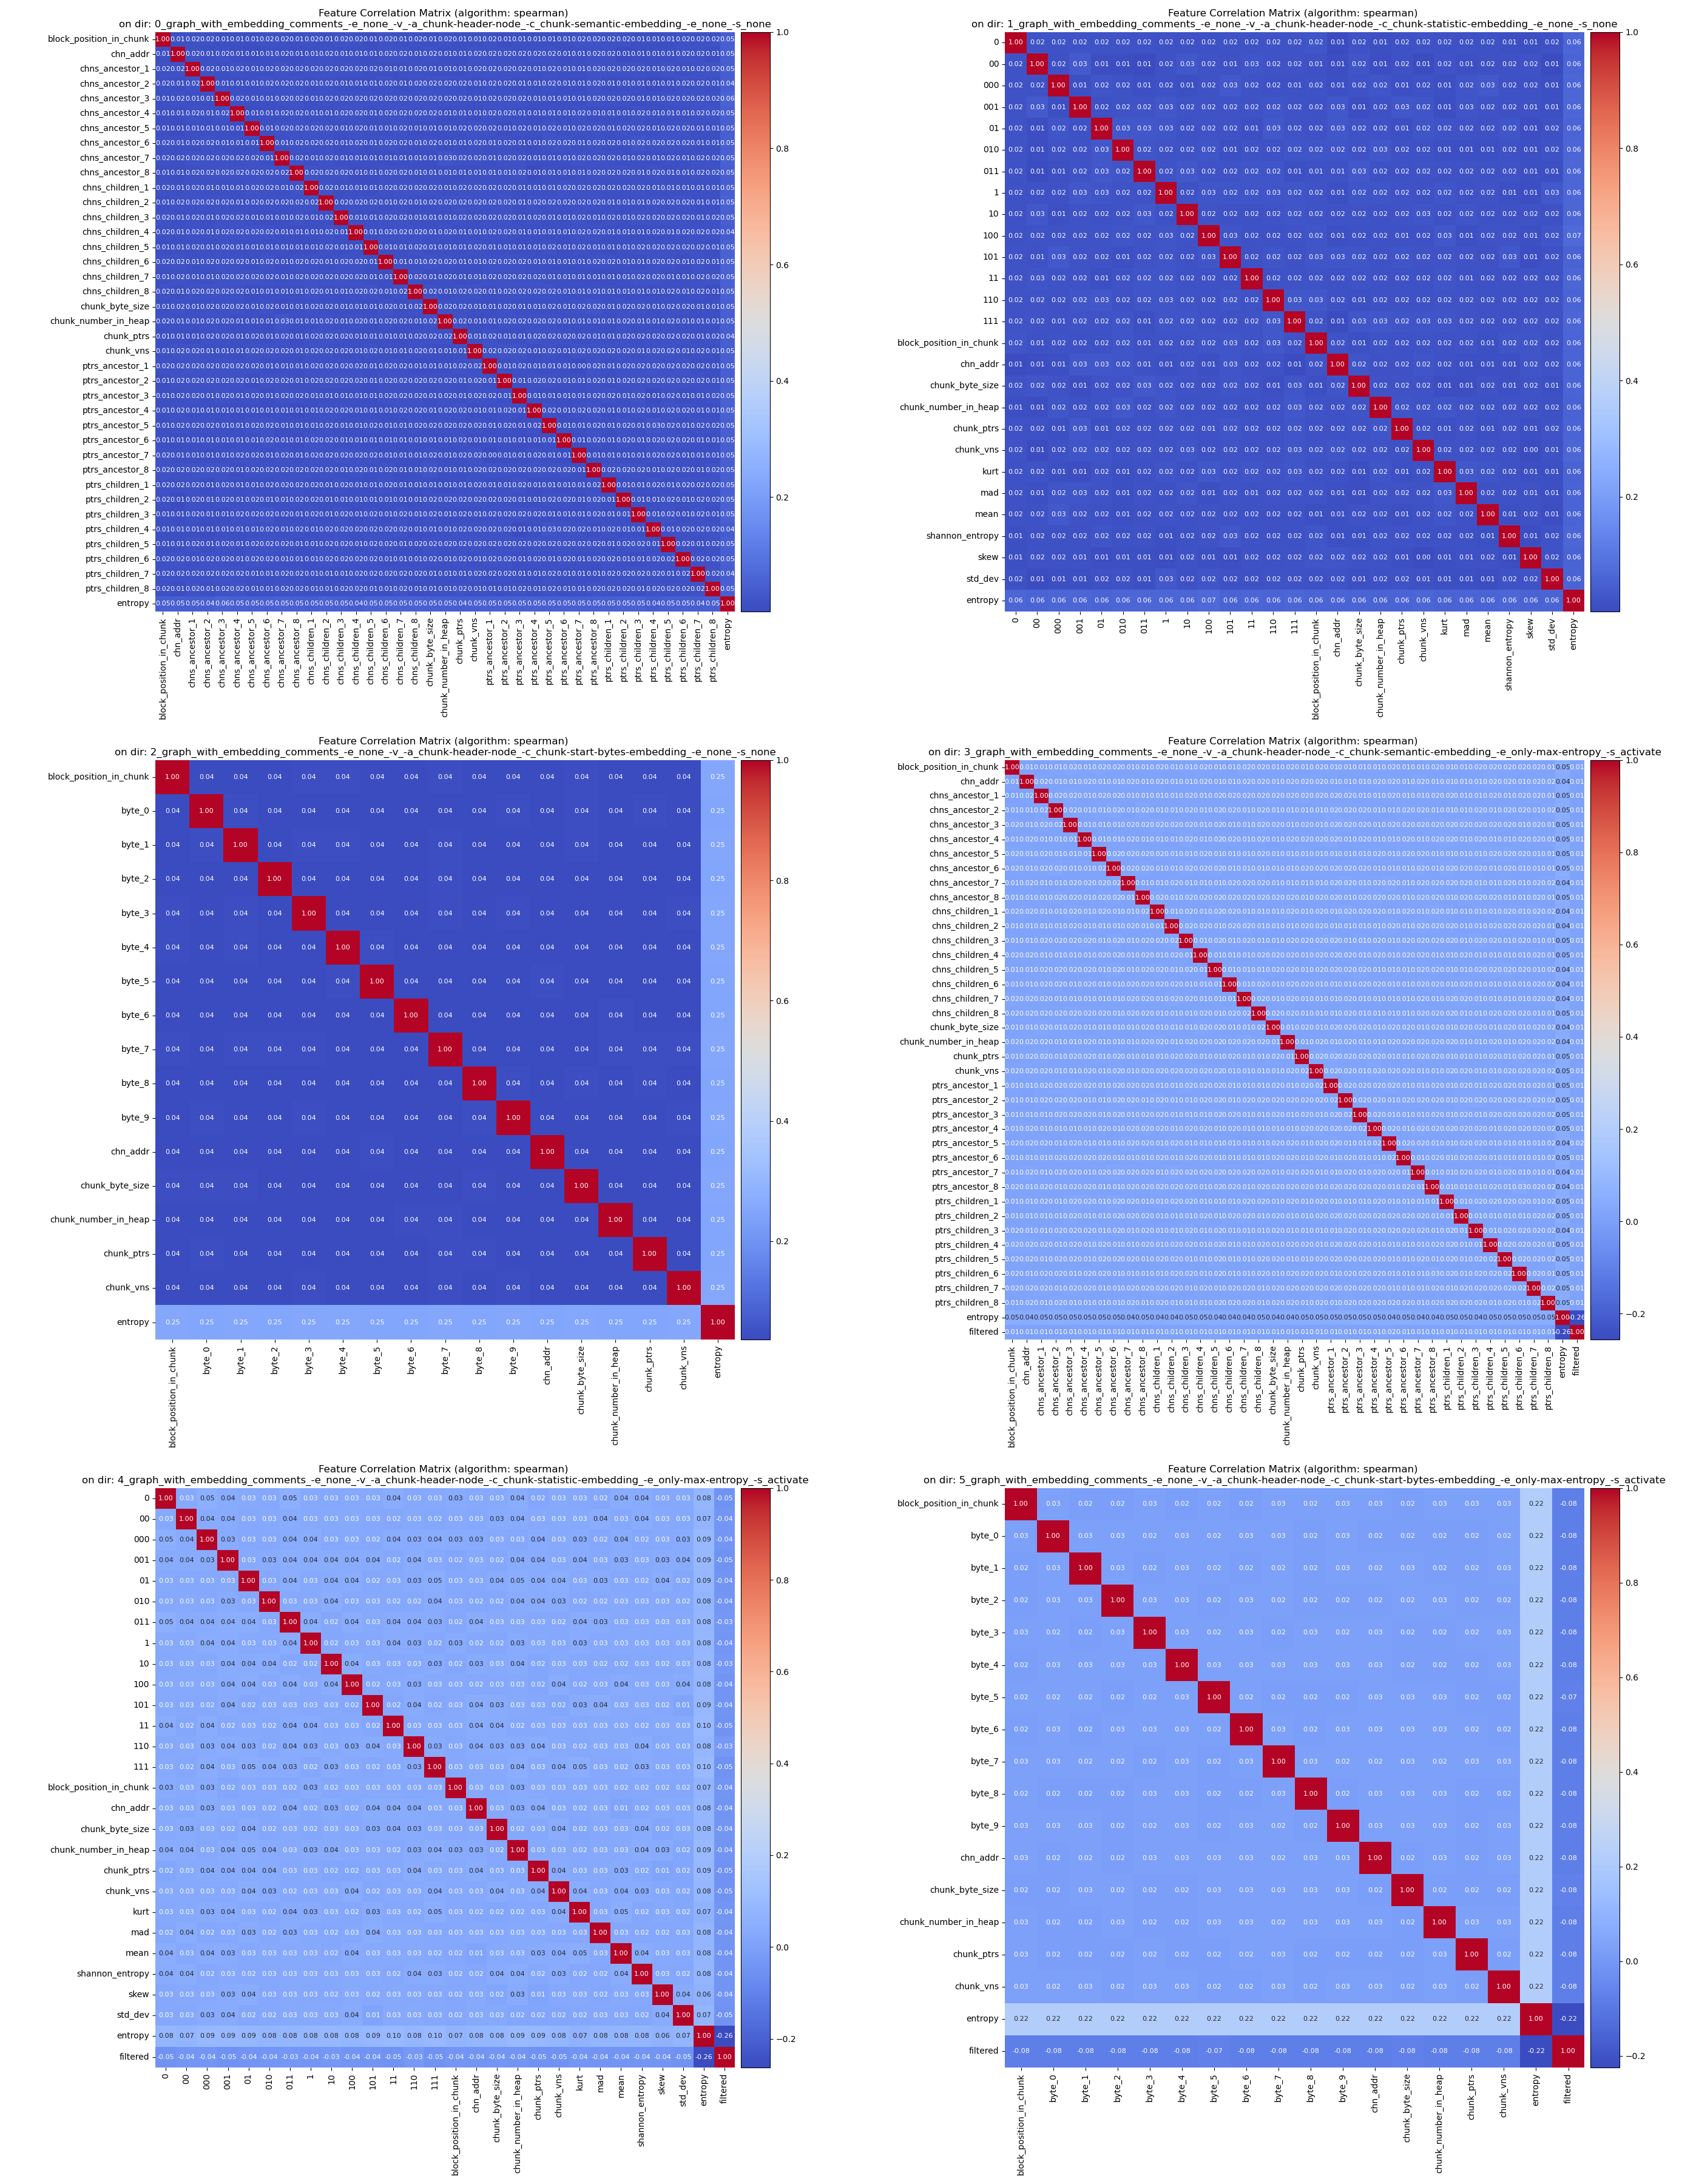
\includegraphics[width=16cm]{feature_engineering/concatenated_3__2023_10_24_spearman.png}
    \caption{Feature correlation matrices on the different Mem2Graph-generated datasets. Used algorithm: Spearman.}
\end{figure}

\section{Classic Model results}

\section{Deep Learning Model results}


